\begin{figure}[H]\centering
    \begin{subfigure}{.3\textwidth}\centering
        \tikzstyle{vertex}=[circle,fill=black,scale=.4]
        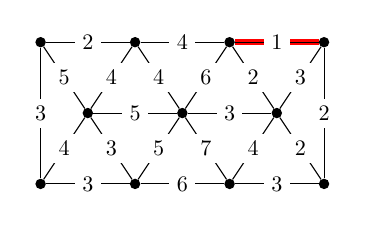
\begin{tikzpicture}[scale=0.3]
    
        \foreach \pos/\name in {{(0,6)/a},{(4,6)/b},{(8,6)/c},{(12,6)/d},
                                {(2,3)/e},{(6,3)/f},{(10,3)/g},
                                {(0,0)/h},{(4,0)/i},{(8,0)/j},{(12,0)/k}}
            \node[vertex] (\name) at \pos {};
        
        \foreach \source/\dest in {c/d}
            \path[draw,red,line width=2pt] (\source) -- node[fill=white,scale=.8] {} (\dest);

        \foreach \source/\dest/\weight in {a/b/2, b/c/4, c/d/1,
                                           a/h/3,a/e/5,e/b/4,b/f/4,f/c/6,c/g/2,g/d/3,d/k/2,
                                           e/f/5,f/g/3,
                                           h/e/4,e/i/3,i/f/5,f/j/7,j/g/4,g/k/2,
                                           h/i/3,i/j/6,j/k/3}
            \path[draw] (\source) -- node[fill=white,scale=.8] {$\weight$} (\dest);
    \end{tikzpicture}
        \caption{}
    \end{subfigure}
    %
    \begin{subfigure}{.3\textwidth}\centering
        \tikzstyle{vertex}=[circle,fill=black,scale=.4]
        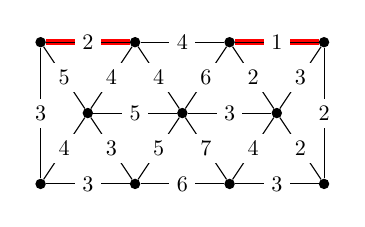
\begin{tikzpicture}[scale=0.3]
    
        \foreach \pos/\name in {{(0,6)/a},{(4,6)/b},{(8,6)/c},{(12,6)/d},
                                {(2,3)/e},{(6,3)/f},{(10,3)/g},
                                {(0,0)/h},{(4,0)/i},{(8,0)/j},{(12,0)/k}}
            \node[vertex] (\name) at \pos {};

         \foreach \source/\dest in {c/d,a/b}
            \path[draw,red,line width=2pt] (\source) -- node[fill=white,scale=.8] {} (\dest);
       
        \foreach \source/\dest/\weight in {a/b/2, b/c/4, c/d/1,
                                           a/h/3,a/e/5,e/b/4,b/f/4,f/c/6,c/g/2,g/d/3,d/k/2,
                                           e/f/5,f/g/3,
                                           h/e/4,e/i/3,i/f/5,f/j/7,j/g/4,g/k/2,
                                           h/i/3,i/j/6,j/k/3}
            \path[draw] (\source) -- node[fill=white,scale=.8] {$\weight$} (\dest);
    \end{tikzpicture}
        \caption{}
    \end{subfigure}
    %
    \begin{subfigure}{.3\textwidth}\centering
        \tikzstyle{vertex}=[circle,fill=black,scale=.4]
        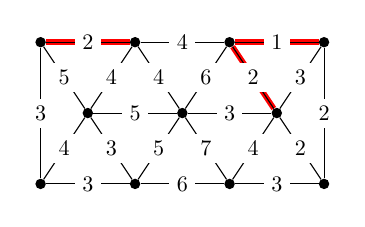
\begin{tikzpicture}[scale=0.3]
    
        \foreach \pos/\name in {{(0,6)/a},{(4,6)/b},{(8,6)/c},{(12,6)/d},
                                {(2,3)/e},{(6,3)/f},{(10,3)/g},
                                {(0,0)/h},{(4,0)/i},{(8,0)/j},{(12,0)/k}}
            \node[vertex] (\name) at \pos {};

         \foreach \source/\dest in {c/d,a/b,c/g}
            \path[draw,red,line width=2pt] (\source) -- node[fill=white,scale=.8] {} (\dest);
       
        \foreach \source/\dest/\weight in {a/b/2, b/c/4, c/d/1,
                                           a/h/3,a/e/5,e/b/4,b/f/4,f/c/6,c/g/2,g/d/3,d/k/2,
                                           e/f/5,f/g/3,
                                           h/e/4,e/i/3,i/f/5,f/j/7,j/g/4,g/k/2,
                                           h/i/3,i/j/6,j/k/3}
            \path[draw] (\source) -- node[fill=white,scale=.8] {$\weight$} (\dest);
    \end{tikzpicture}
        \caption{}
    \end{subfigure}
    %
    \begin{subfigure}{.3\textwidth}\centering
        \tikzstyle{vertex}=[circle,fill=black,scale=.4]
        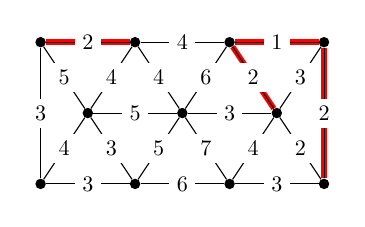
\begin{tikzpicture}[scale=0.3]
    
        \foreach \pos/\name in {{(0,6)/a},{(4,6)/b},{(8,6)/c},{(12,6)/d},
                                {(2,3)/e},{(6,3)/f},{(10,3)/g},
                                {(0,0)/h},{(4,0)/i},{(8,0)/j},{(12,0)/k}}
            \node[vertex] (\name) at \pos {};

         \foreach \source/\dest in {c/d,a/b,c/g,d/k}
            \path[draw,red,line width=2pt] (\source) -- node[fill=white,scale=.8] {} (\dest);
       
        \foreach \source/\dest/\weight in {a/b/2, b/c/4, c/d/1,
                                           a/h/3,a/e/5,e/b/4,b/f/4,f/c/6,c/g/2,g/d/3,d/k/2,
                                           e/f/5,f/g/3,
                                           h/e/4,e/i/3,i/f/5,f/j/7,j/g/4,g/k/2,
                                           h/i/3,i/j/6,j/k/3}
            \path[draw] (\source) -- node[fill=white,scale=.8] {$\weight$} (\dest);
    \end{tikzpicture}
        \caption{}
    \end{subfigure}
    %
    \begin{subfigure}{.3\textwidth}\centering
        \tikzstyle{vertex}=[circle,fill=black,scale=.4]
        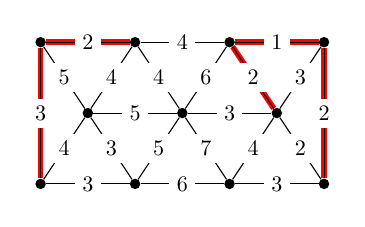
\begin{tikzpicture}[scale=0.3]
    
        \foreach \pos/\name in {{(0,6)/a},{(4,6)/b},{(8,6)/c},{(12,6)/d},
                                {(2,3)/e},{(6,3)/f},{(10,3)/g},
                                {(0,0)/h},{(4,0)/i},{(8,0)/j},{(12,0)/k}}
            \node[vertex] (\name) at \pos {};

         \foreach \source/\dest in {c/d,a/b,c/g,d/k,a/h}
            \path[draw,red,line width=2pt] (\source) -- node[fill=white,scale=.8] {} (\dest);
       
        \foreach \source/\dest/\weight in {a/b/2, b/c/4, c/d/1,
                                           a/h/3,a/e/5,e/b/4,b/f/4,f/c/6,c/g/2,g/d/3,d/k/2,
                                           e/f/5,f/g/3,
                                           h/e/4,e/i/3,i/f/5,f/j/7,j/g/4,g/k/2,
                                           h/i/3,i/j/6,j/k/3}
            \path[draw] (\source) -- node[fill=white,scale=.8] {$\weight$} (\dest);
    \end{tikzpicture}
        \caption{}
    \end{subfigure}
       %
    \begin{subfigure}{.3\textwidth}\centering
        \tikzstyle{vertex}=[circle,fill=black,scale=.4]
        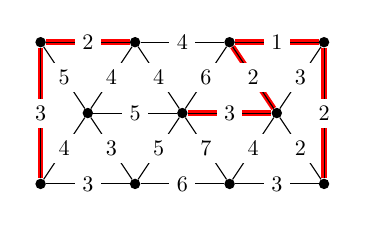
\begin{tikzpicture}[scale=0.3]
    
        \foreach \pos/\name in {{(0,6)/a},{(4,6)/b},{(8,6)/c},{(12,6)/d},
                                {(2,3)/e},{(6,3)/f},{(10,3)/g},
                                {(0,0)/h},{(4,0)/i},{(8,0)/j},{(12,0)/k}}
            \node[vertex] (\name) at \pos {};

         \foreach \source/\dest in {c/d,a/b,c/g,d/k,a/h,f/g}
            \path[draw,red,line width=2pt] (\source) -- node[fill=white,scale=.8] {} (\dest);
       
        \foreach \source/\dest/\weight in {a/b/2, b/c/4, c/d/1,
                                           a/h/3,a/e/5,e/b/4,b/f/4,f/c/6,c/g/2,g/d/3,d/k/2,
                                           e/f/5,f/g/3,
                                           h/e/4,e/i/3,i/f/5,f/j/7,j/g/4,g/k/2,
                                           h/i/3,i/j/6,j/k/3}
            \path[draw] (\source) -- node[fill=white,scale=.8] {$\weight$} (\dest);
    \end{tikzpicture}
        \caption{}
    \end{subfigure}
   %
    \begin{subfigure}{.3\textwidth}\centering
        \tikzstyle{vertex}=[circle,fill=black,scale=.4]
        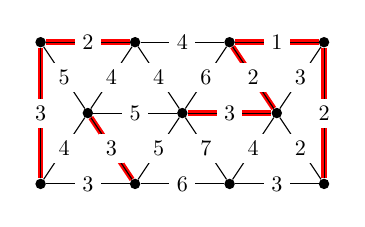
\begin{tikzpicture}[scale=0.3]
    
        \foreach \pos/\name in {{(0,6)/a},{(4,6)/b},{(8,6)/c},{(12,6)/d},
                                {(2,3)/e},{(6,3)/f},{(10,3)/g},
                                {(0,0)/h},{(4,0)/i},{(8,0)/j},{(12,0)/k}}
            \node[vertex] (\name) at \pos {};

         \foreach \source/\dest in {c/d,a/b,c/g,d/k,a/h,f/g,e/i}
            \path[draw,red,line width=2pt] (\source) -- node[fill=white,scale=.8] {} (\dest);
       
        \foreach \source/\dest/\weight in {a/b/2, b/c/4, c/d/1,
                                           a/h/3,a/e/5,e/b/4,b/f/4,f/c/6,c/g/2,g/d/3,d/k/2,
                                           e/f/5,f/g/3,
                                           h/e/4,e/i/3,i/f/5,f/j/7,j/g/4,g/k/2,
                                           h/i/3,i/j/6,j/k/3}
            \path[draw] (\source) -- node[fill=white,scale=.8] {$\weight$} (\dest);
    \end{tikzpicture}
        \caption{}
    \end{subfigure}
   %
    \begin{subfigure}{.3\textwidth}\centering
        \tikzstyle{vertex}=[circle,fill=black,scale=.4]
        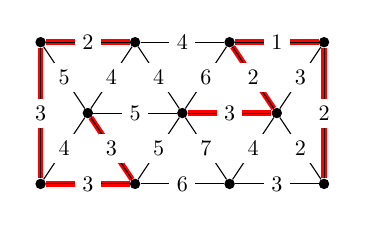
\begin{tikzpicture}[scale=0.3]
    
        \foreach \pos/\name in {{(0,6)/a},{(4,6)/b},{(8,6)/c},{(12,6)/d},
                                {(2,3)/e},{(6,3)/f},{(10,3)/g},
                                {(0,0)/h},{(4,0)/i},{(8,0)/j},{(12,0)/k}}
            \node[vertex] (\name) at \pos {};

         \foreach \source/\dest in {c/d,a/b,c/g,d/k,a/h,f/g,e/i,h/i}
            \path[draw,red,line width=2pt] (\source) -- node[fill=white,scale=.8] {} (\dest);
       
        \foreach \source/\dest/\weight in {a/b/2, b/c/4, c/d/1,
                                           a/h/3,a/e/5,e/b/4,b/f/4,f/c/6,c/g/2,g/d/3,d/k/2,
                                           e/f/5,f/g/3,
                                           h/e/4,e/i/3,i/f/5,f/j/7,j/g/4,g/k/2,
                                           h/i/3,i/j/6,j/k/3}
            \path[draw] (\source) -- node[fill=white,scale=.8] {$\weight$} (\dest);
    \end{tikzpicture}
        \caption{}
    \end{subfigure}
   %
    \begin{subfigure}{.3\textwidth}\centering
        \tikzstyle{vertex}=[circle,fill=black,scale=.4]
        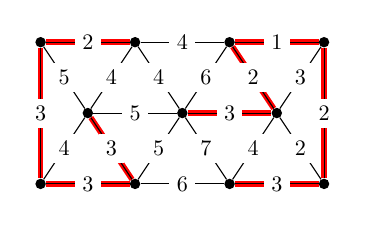
\begin{tikzpicture}[scale=0.3]
    
        \foreach \pos/\name in {{(0,6)/a},{(4,6)/b},{(8,6)/c},{(12,6)/d},
                                {(2,3)/e},{(6,3)/f},{(10,3)/g},
                                {(0,0)/h},{(4,0)/i},{(8,0)/j},{(12,0)/k}}
            \node[vertex] (\name) at \pos {};

         \foreach \source/\dest in {c/d,a/b,c/g,d/k,a/h,f/g,e/i,h/i,j/k}
            \path[draw,red,line width=2pt] (\source) -- node[fill=white,scale=.8] {} (\dest);
       
        \foreach \source/\dest/\weight in {a/b/2, b/c/4, c/d/1,
                                           a/h/3,a/e/5,e/b/4,b/f/4,f/c/6,c/g/2,g/d/3,d/k/2,
                                           e/f/5,f/g/3,
                                           h/e/4,e/i/3,i/f/5,f/j/7,j/g/4,g/k/2,
                                           h/i/3,i/j/6,j/k/3}
            \path[draw] (\source) -- node[fill=white,scale=.8] {$\weight$} (\dest);
    \end{tikzpicture}
        \caption{}
    \end{subfigure}   %
    \begin{subfigure}{.3\textwidth}\centering
        \tikzstyle{vertex}=[circle,fill=black,scale=.4]
        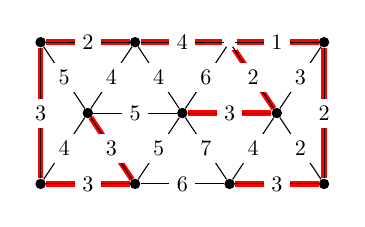
\begin{tikzpicture}[scale=0.3]
    
        \foreach \pos/\name in {{(0,6)/a},{(4,6)/b},{(8,6)/c},{(12,6)/d},
                                {(2,3)/e},{(6,3)/f},{(10,3)/g},
                                {(0,0)/h},{(4,0)/i},{(8,0)/j},{(12,0)/k}}
            \node[vertex] (\name) at \pos {};

         \foreach \source/\dest in {c/d,a/b,c/g,d/k,a/h,f/g,e/i,h/i,j/k,b/d}
            \path[draw,red,line width=2pt] (\source) -- node[fill=white,scale=.8] {} (\dest);
       
        \foreach \source/\dest/\weight in {a/b/2, b/c/4, c/d/1,
                                           a/h/3,a/e/5,e/b/4,b/f/4,f/c/6,c/g/2,g/d/3,d/k/2,
                                           e/f/5,f/g/3,
                                           h/e/4,e/i/3,i/f/5,f/j/7,j/g/4,g/k/2,
                                           h/i/3,i/j/6,j/k/3}
            \path[draw] (\source) -- node[fill=white,scale=.8] {$\weight$} (\dest);
    \end{tikzpicture}
        \caption{}
    \end{subfigure}
\end{figure}
